\section{Node Union Reference}
\label{union_node}\index{Node@{Node}}
Collaboration diagram for Node:\begin{figure}[H]
\begin{center}
\leavevmode
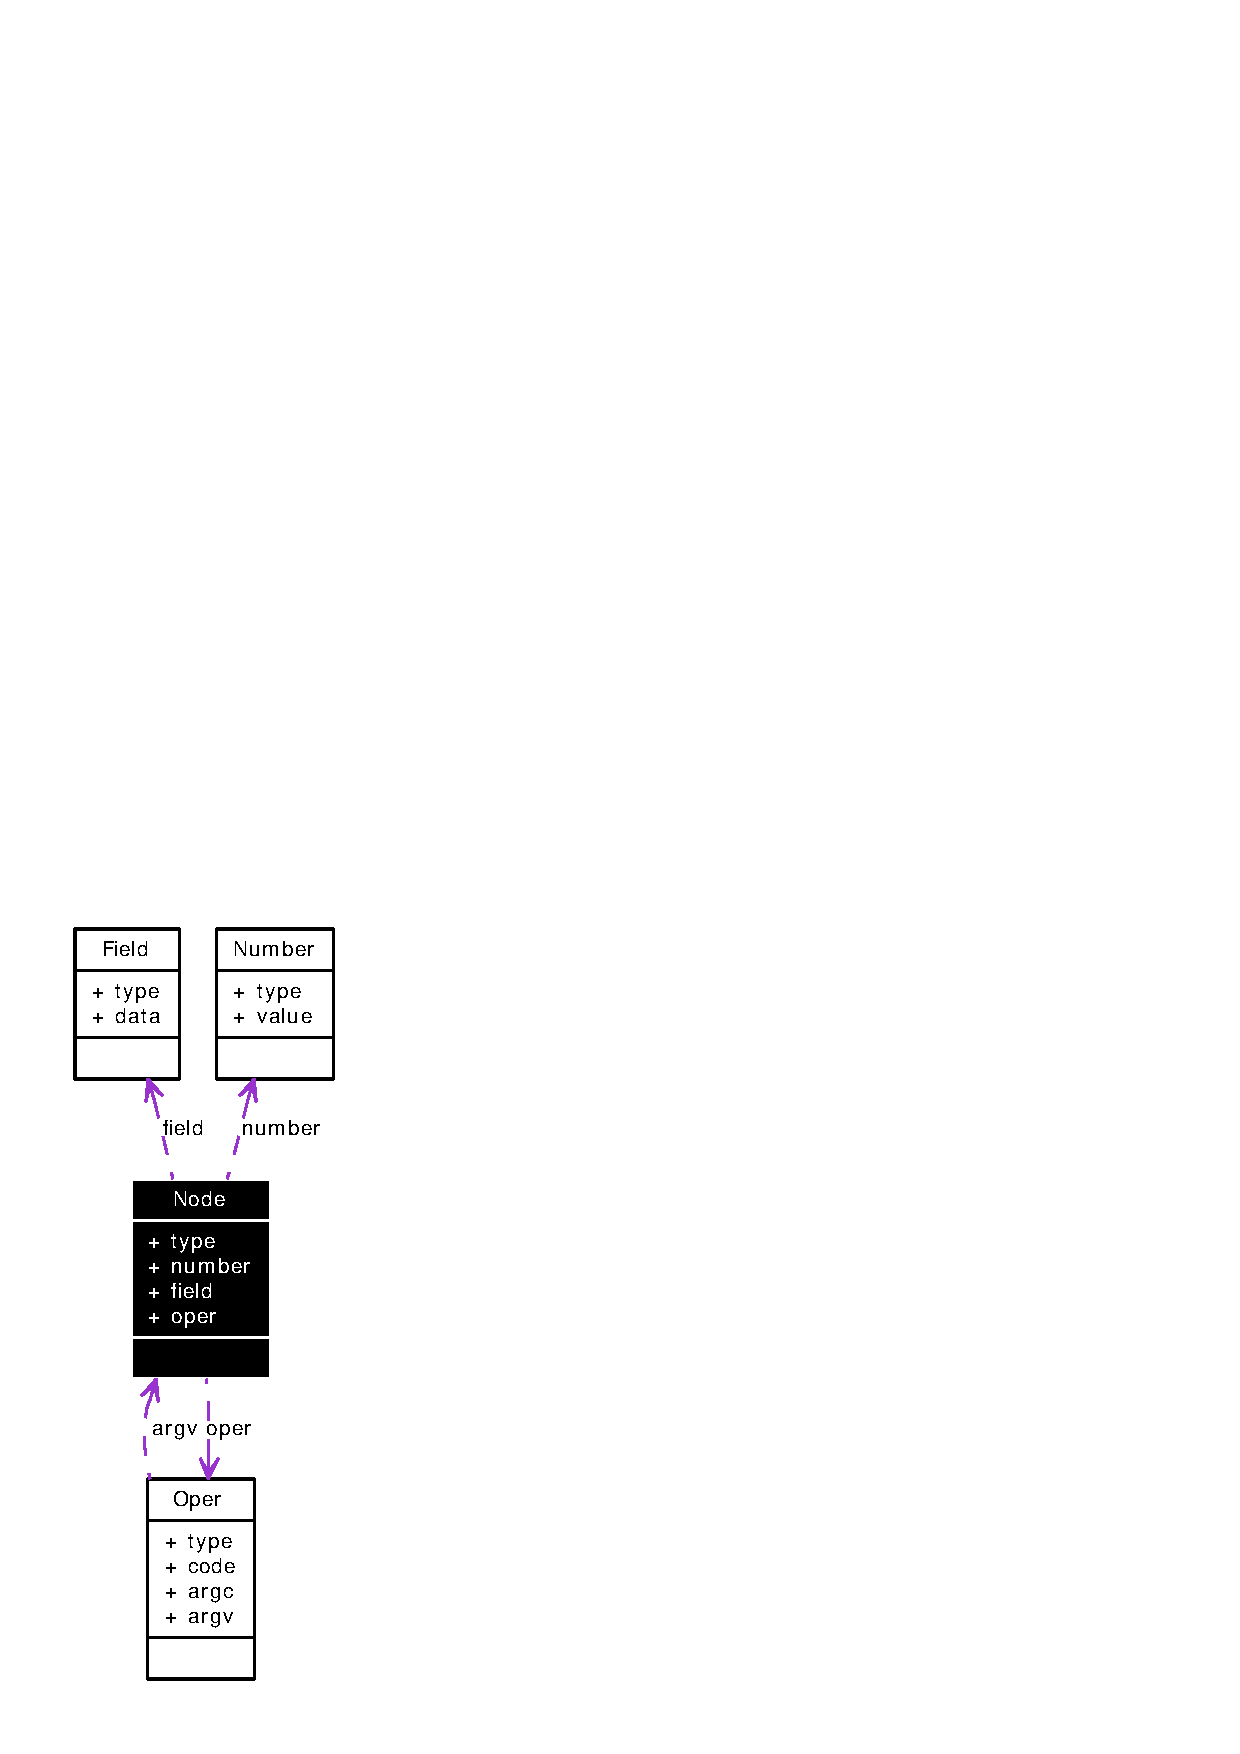
\includegraphics[width=86pt]{union_node__coll__graph}
\end{center}
\end{figure}
\subsection*{Public Attributes}
\begin{CompactItemize}
\item 
Type {\bf type}\label{union_node_o0}

\item 
{\bf Number} {\bf number}\label{union_node_o1}

\item 
{\bf Field} {\bf field}\label{union_node_o2}

\item 
{\bf Oper} {\bf oper}\label{union_node_o3}

\end{CompactItemize}


\subsection{Detailed Description}




Definition at line 120 of file calc.tab.cpp.

The documentation for this union was generated from the following file:\begin{CompactItemize}
\item 
calc.tab.cpp\end{CompactItemize}
